% Standalone figure: dual-gate vs. single-threshold CRC baseline.
% source: data/crcbaseline.csv <- baseline_comparison_2026-07-15/results.json
%   (benchmarks.{MPDD,VisA,MVTec-AD}.{our_gate_published,crc_baseline}, pooled
%   over both backbones and five seeds; identical to manuscripts Table
%   \ref{tab:crcbaseline}). No values recomputed here -- transcribed from the
%   frozen JSON and cross-checked against the manuscript table text.
% Compile: pdflatex fig-crcbaseline.tex  (see Makefile)
\documentclass[border=1pt]{standalone}
\usepackage[T1]{fontenc}
\usepackage{pgfplots}
\pgfplotsset{compat=1.18}
\usepackage{pgfplotstable}
\usetikzlibrary{patterns}

% Colorblind-safe qualitative palette (Okabe-Ito subset).
\definecolor{cEscaped}{HTML}{0072B2}   % blue
\definecolor{cFalseReject}{HTML}{D55E00} % vermillion
\definecolor{cDeferral}{HTML}{009E73}   % bluish green

\begin{document}
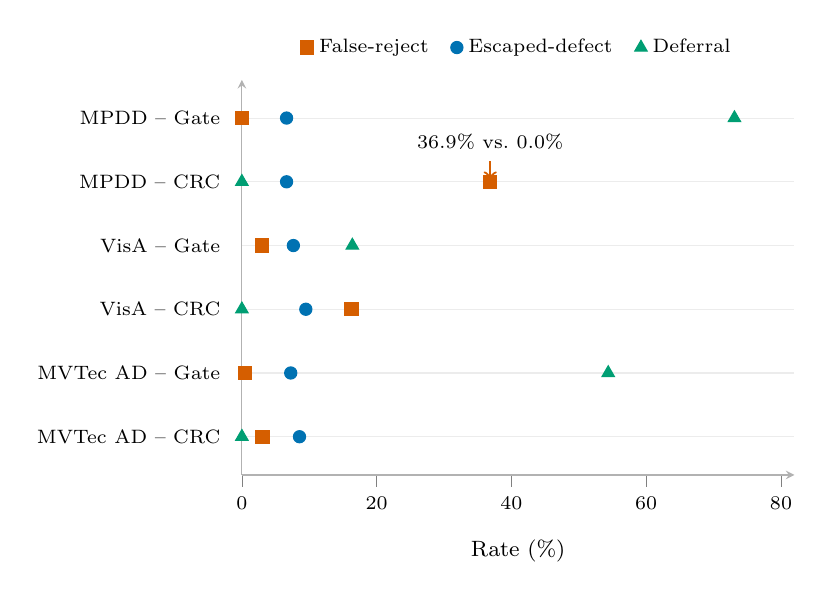
\begin{tikzpicture}[font=\fontsize{8}{9.5}\selectfont]
\begin{axis}[
    width=8.6cm, height=6.6cm,
    xmin=0, xmax=82,
    ymin=0.4, ymax=6.6,
    xlabel={Rate (\%)},
    xlabel style={font=\fontsize{8}{9.5}\selectfont},
    x label style={at={(axis description cs:0.5,-0.14)}},
    axis x line=bottom,
    axis y line=left,
    ytick={1,2,3,4,5,6},
    yticklabels={
      {MVTec AD -- CRC},
      {MVTec AD -- Gate},
      {VisA -- CRC},
      {VisA -- Gate},
      {MPDD -- CRC},
      {MPDD -- Gate}
    },
    y tick label style={font=\fontsize{7.5}{8.5}\selectfont, align=right},
    x tick label style={font=\fontsize{7.5}{8.5}\selectfont},
    tick align=outside,
    ytick style={draw=none},
    every axis plot/.append style={mark options={scale=1.0}},
    ymajorgrids, grid style={gray!15},
    axis line style={gray!60},
    legend style={
      at={(0.5,1.03)}, anchor=south, legend columns=3,
      font=\fontsize{7.5}{8.5}\selectfont, draw=none, fill=none,
      /tikz/every even column/.append style={column sep=6pt}
    },
    clip=false,
]

% ---- False-reject (the headline contrast): draw first so the guide bar sits behind markers.
\addplot[cFalseReject, only marks, mark=square*, mark size=2.4pt] coordinates {
  (36.85,5) (0.00,6) (16.24,3) (2.96,4) (3.06,1) (0.46,2)
};
\addlegendentry{False-reject}

% ---- Escaped-defect.
\addplot[cEscaped, only marks, mark=*, mark size=2.2pt] coordinates {
  (6.63,5) (6.63,6) (9.49,3) (7.64,4) (8.55,1) (7.25,2)
};
\addlegendentry{Escaped-defect}

% ---- Deferral.
\addplot[cDeferral, only marks, mark=triangle*, mark size=2.6pt] coordinates {
  (0.00,5) (73.09,6) (0.00,3) (16.39,4) (0.00,1) (54.36,2)
};
\addlegendentry{Deferral}

% Callout on the MPDD false-reject contrast.
\draw[cFalseReject, thick, ->] (axis cs:36.85,5.32) -- (axis cs:36.85,5.05);
\node[black, font=\fontsize{7}{8}\selectfont, anchor=south, align=center] at (axis cs:36.85,5.36) {$36.9\%$ vs.\ $0.0\%$};

\end{axis}
\end{tikzpicture}
\end{document}
